% ============================================================
%  chapters/proposal_body.tex —— 开题报告正文（官方表格 4 节结构）
%
%  内容源：thesis/proposal.md（由本文件经 scripts/tex2md.py 生成的可编辑镜像）
%  v3（2026-11-03）按任务书 v6 与导师意见改写：
%    1. 删去一.1 的“课题基本信息”表（封面已含，任务书 v6 亦不再单列）；
%    2. 一.2 由“国内外研究现状和发展趋势”改为“文献综述”，按五条脉络重排，
%       原一.1 的智能体能力文献移入综述第（一）节，正文引用顺序保持 [1]—[44]；
%    3. 二.2 改为“初步实施方案”，按理论研究、数据模型、算法方法、原型功能、
%       评估验证五个模块作学术化论述，删去四层架构、风险表、人日工作量、
%       可行性清单等软工报告式内容；进度表按任务书 v6 的 6 阶段教学周重排。
%
%  图表编号：由 \tjformsecnum{n} 按一级小节号接管（图 2-1、表 2-1 …）；
%  正文交叉引用一律 \ref，不写旧稿的图 6-1 / 表 10-1 等编号。
%
%  摘要块：官方开题报告表格无“摘要”栏；本课题保留原稿摘要以便与 Word 版对照，
%  由 \iftjproposalabstract 开关控制（定义于 chapters/tj-extras.tex）。
%  学院若不允许摘要，删除下面 \iftjproposalabstract … \fi 之间的内容即可
%  （开关本身保留，不影响编译）。
% ============================================================

% ---- PDF 链接锚点：\tjformsecnum 重定义了 \thetable/\thefigure，但 hyperref 的
% \theHtable/\theHfigure 仍按 chapter 计数（无 chapter 时恒为 0.1），图表共用同一
% 锚点，xdvipdfmx 因此报 "Object @table.0.1 already defined"。让 H 锚点跟随显示编号。
\makeatletter
\renewcommand{\theHtable}{\thetable}
\renewcommand{\theHfigure}{\thefigure}
\makeatother

\iftjproposalabstract
\tjformsection{摘要}

开发者借助代码智能体完成代码修改、执行与测试已成为常态，但对话、变更、工具调用与测试结果分散在不同界面，缺少以开发任务为中心的组织，使“为何这样修改、依据什么验证、中断后如何接续”难以回答。本课题面向单个开发者，研究任务、对话、变更、工具调用与测试之间的关联与组织方法，设计并实现支持任务上下文追踪与变更溯源的 Web 原型，并从理论研究、数据模型、算法方法、原型功能与评估验证五个方面提出初步实施方案。本研究定位为小样本探索性预研，结论以 6—8 个任务与 4—5 名受试者的描述统计结果表述。

\textbf{关键词}：代码智能体；任务上下文；变更溯源；中断恢复；证据链
\fi

\tjformsection{一、\tjheadertext 课题背景}\tjformsecnum{1}

\tjformsubsection{1．课题来源及研究的目的和意义}

近年来，代码智能体（code agent）逐渐应用于日常软件开发。开发者以自然语言描述任务，由智能体完成代码分析、文件修改、工具调用、测试执行与问题排查。与代码补全不同，智能体的产出并非一段建议代码，而是一组带有工具调用与执行反馈的操作序列；开发过程由此从“人写代码”转变为“人下指令、智能体实施、人审查验证”的协作过程。这一转变在提高任务吞吐的同时，也使“过程是否可理解、可核查、可接续”成为开发者必须面对的问题。

然而，现有工具通常将过程信息分散于不同界面或不同类型的记录之中：对话留存于会话窗口，代码差异留存于 diff 视图，工具调用留存于终端日志，测试结果留存于测试报告，版本演化留存于 Git 历史。这些记录之间既缺少共同标识，也缺少以开发任务为中心的组织。由此产生三方面问题：一是任务视角缺失，在多轮修改、多任务并行与中断重启后难以掌握当前进展；二是溯源断裂，代码因何而改、依据哪次测试验证，只能依靠人工查找与回忆；三是上下文丢失，重新开始工作时需重读长对话与大量差异。

本课题面向单个开发者使用代码智能体完成开发任务的场景，研究开发任务、对话、代码变更、工具调用与测试结果之间的关联与组织方法，设计并实现支持任务上下文追踪与变更溯源的 Web 原型，使开发者能够围绕任务、文件或代码片段审视“为何修改、依据何在、验证结果如何”，并在任务中断后恢复必要的上下文。

本课题的意义体现在三个层面。理论层面，将“任务上下文”与“变更溯源”的概念从 IDE 与桌面场景迁移至智能体驱动的“指令—工具调用—变更—测试”序列，建立其与 PROV 的映射，并讨论任务边界判定、异构记录关联与证据充分性等表示问题。实践层面，将关联、溯源与恢复实现为可查询、可复现的原型，为单个开发者提供可操作的证据链，而非停留于日志浏览。教学层面，完整经历“问题识别—文献定位—模型设计—原型实现—实证评估”的研究流程，并明确说明小样本评估结论的适用边界。

\tjformsubsection{2．文献综述}

本节按“代码智能体与软件工程自动化—变更分析与代码历史—任务上下文与中断恢复—过程溯源与证据链—工程工具现状”五条脉络梳理相关研究，并在此基础上进行述评。文献检索以 Google Scholar、DBLP、arXiv、ACM Digital Library 与《软件学报》为主，检索词包括 code agent、software engineering agent、task context、provenance、program comprehension、resumption 等。

\tjformsubsub{（一）代码智能体与软件工程自动化}

SWE-bench 以真实 GitHub issue 检验端到端修复，该文报告当时最优模型仅解决 1.96\% 的任务[1]；针对代码生成能力的系统评测则提供了更一般的基准结果[2]。此后，SWE-agent[3]、OpenHands[4] 与 CodeAct[5] 等以工具调用与执行反馈为核心的方法明显提升了该指标；MetaGPT[6] 与 ChatDev[7] 探索多智能体协作，亦有研究主张以更简化的流程取得可比效果[8]。相关综述从软件工程全流程[9-10]、检索增强[11]与测试生成[12]等角度总结了研究进展。

能力提升并未消除使用成本。一项对照实验报告称，Copilot 使任务完成速度提升约 55.8\%[13]，但开发者仍需进行额外审查与验证[14-15]，且在采纳生成代码前通常需先理解并验证其行为[16-17]。更为重要的是，现有评价多以最终修复率或生成质量为指标，过程证据——哪条指令触发修改、哪次工具调用实施修改、哪次测试完成验证——并不在评价范围之内。这表明：智能体的产出若要被开发者信任并接续，必须伴随可核查的过程证据。

\tjformsubsub{（二）变更分析与代码历史}

软件仓库挖掘为变更与问题之间的关联提供了方法基础：SZZ 依据修复提交所引用的缺陷报告回溯引入缺陷的变更[18]，Kagdi 等综述了仓库挖掘的任务与方法[19]，Robbes 与 Lanza 主张以变更为中心分析软件演化[20]；GumTree 通过语法树差分生成比行级 diff 更精确的变更脚本[21]，CodeShovel 重建方法级代码历史[22]。上述方法回答了“改了什么”，其关联对象是提交与缺陷报告，而非“由哪条指令触发、由哪次测试验证”。

\tjformsubsub{（三）任务上下文与中断恢复}

以任务为单位组织开发上下文并非新的研究命题。Mylyn 提出任务上下文模型，通过任务聚焦界面按当前任务过滤 IDE 代码元素[23]；TaskTracer 在桌面环境中将文件、邮件与网页归集到任务[24]；ActivitySpace 跨应用推荐相关代码元素[25]；Codebook 建立代码实体与提交、缺陷、邮件之间的关联图[26]。在中断恢复方面，Parnin 与 Rugaber 归纳了恢复策略对线索丰富度的依赖[27]，Parnin 与 DeLine 通过受控实验比较了情景线索与语义线索[28]，Safer 与 Murphy 研究了任务边界识别界面[29]，Robbes 与 Lanza 刻画了开发会话的结构[30]。上述工作构成本课题的基础，但其前提是开发者直接在 IDE 或桌面环境中操作、任务由开发者显式声明，线索主要来自编辑与窗口事件；在智能体事件流中，任务边界通常未被显式声明，线索形态也由文本、工具调用与执行结果构成。

\tjformsubsub{（四）过程溯源与证据链}

数据库领域提出了溯源的经典框架[31]；PROV-O 将溯源抽象为实体、活动与代理及其派生关系，已成为跨系统交换标准[32]；PROV-AGENT 覆盖智能体交互中的提示、响应、决策与工具调用[33]。Whyline 通过“为什么”式提问组织执行证据[34]，noWorkflow 将脚本执行过程捕获为可查询的溯源图[35]。上述工作证明了证据链的价值，但尚未面向“指令—工具调用—变更—测试”这一异构序列建模，也未将验证依据纳入证据图。

\tjformsubsub{（五）工程工具现状与研究述评}

工程实践中已有工具亦可归入上述方向：智能体客户端（Claude Code[36]、Cursor[37]、Cline[38]）以会话或文件为单位提供历史记录与检查点，但检查点随会话结束或保留期届满而失效；LLM 可观测性平台（Langfuse[39]）与 OpenTelemetry 生成式 AI 语义约定[40] 记录调用链与耗时，未与代码变更、测试结果进行语义对齐。

上述工作可归为四个方向：智能体能力、变更分析、任务上下文与中断恢复、过程溯源。四者均有所积累，但尚未同时满足以下三点：（1）以任务为根节点统一关联对话、变更、工具调用与测试；（2）变更粒度达到 hunk 并支持双向查询；（3）在证据绑定约束下利用大模型生成摘要与进展整理。需要说明的是，“以任务为单位组织上下文”本身并非研究空白，Mylyn[23] 与 Parnin 等[27-28] 已提供模型与实证基础；本课题的差异在于研究对象从“人在 IDE 中的编辑事件”转变为“智能体驱动的指令—工具调用—变更—测试序列”，并将验证依据纳入证据链。在所及文献范围内，尚未见到同时满足上述三点的系统；文献综述定稿阶段将补充系统检索，并记录检索式与命中数。

\tjformsection{二、\tjheadertext 方案介绍}\tjformsecnum{2}

\tjformsubsection{1．研究问题与研究内容}

本课题围绕“单个开发者使用代码智能体时，开发过程信息如何被组织、溯源与恢复”这一核心问题，将其分解为五个可检验的研究问题。

RQ1（表示）：统一事件模型能否在不修改采集端的前提下，覆盖一种真实代码智能体来源（Claude Code）以及 Git 与测试记录的全部类型？以事件类型覆盖率与文件级位置映射成功率度量。

RQ2（关联）：融合时间邻近、显式引用与文件级位置映射的关联方法，在 20—30 对人工核对样本上的关联准确率达到何种水平？

RQ3（溯源）：以 hunk 为粒度、绑定触发消息与验证测试的证据链，能否在 15 条预注册查询上达到可接受的命中率？大模型摘要的弃答率与不支持率处于何种水平？

RQ4（续接）：由进展摘要、未完成项与待验证修改构成的最小上下文，能否减少 4—5 名受试者的恢复用时并提高理解要点命中数？SUS 评分处于何种水平？

RQ5（边界）：基于空闲时长、显式指令与提交动作的边界判定规则，在 6—8 个任务上的 F1 达到何种水平？阈值对结果的影响程度如何？

围绕上述问题，本课题的研究内容分为五项，覆盖任务书“应完成的主要内容”中信息模型、原型系统与实验评估等要求。（1）信息模型与统一事件表示：抽象出开发任务、对话轮次、消息、工具调用、文件变更（hunk）、测试运行、测试用例结果与检查点八类实体及其关系，设计可扩展事件模式与存储结构，并建立其与 PROV-O 的映射。（2）上下文采集与关联：接入 Claude Code 的会话与工具调用、文件系统与 Git、测试报告，将编辑动作归一化为 hunk；研究基于时间邻近、显式引用与文件级位置映射的多对多关联，并判定任务边界。（3）变更溯源与证据链：以 hunk 为单位生成变更卡片，记录触发来源、实施过程、修改前后快照、验证依据与后续演化，支持“代码—原因—证据”的 1—2 跳双向查询。（4）交互界面与任务续接：实现任务中心、任务时间线与变更证据侧栏三个视图；任务中断后生成任务快照，呈现已完成、未完成与待验证事项，并支持由快照跳转至证据。（5）大语言模型辅助与评估：生成任务摘要、整理开发进展，要求输出绑定证据标识，证据不足时弃答；在 6—8 个典型任务与 4—5 名受试者上评估系统在代码理解、修改原因分析、问题定位与任务衔接方面的作用。

研究边界如下：本课题不实现或训练代码智能体本身，不构建通用 LLM 可观测性平台，不涉及云端多租户、团队协作、跨仓库聚合与多智能体调度；界面限定为 Web 形态的三个核心视图，文件与代码片段视角作为时间线的过滤与详情呈现；IDE 插件与第二来源适配列为可选，不计入必做范围。

本课题的创新点主要有四项。第一，面向智能体会话的任务上下文重建：不依赖显式任务声明，依据空闲时长、目标切换、显式指令与提交动作判定任务边界，将跨会话的对话、变更、工具调用与测试归并至同一任务；与 Mylyn[23] 等以“显式激活任务 + IDE 代码元素”为前提的界面不同。第二，含验证依据的细粒度变更证据链：以 hunk 为单位同时绑定触发消息、工具调用、测试运行与后续演化，回答“为何修改、依据何在、是否仍然有效”；SZZ[18] 与 Codebook[26] 主要建立单向或静态关联。第三，面向中断恢复的恢复快照自动生成：将恢复线索的获取从人工重建转为由任务上下文图自动生成，以任务快照呈现三类事项并支持跳转至证据；已有研究[27-28] 提供了线索类型与策略，但所需信息仍需人工搜集。第四，受证据绑定约束的大模型辅助：每条摘要与进展结论均绑定真实证据标识，证据不足时弃答，并并列报告弃答率与不支持率，以避免以少答换取低错误率。

预期成果包括：一套可运行的原型系统（含源代码、部署与使用说明，支持离线模式）；毕业设计（论文）一份；系统设计、测试与评估报告，实验数据与复现脚本；经脱敏的开发过程事件样例数据集（不少于 300 条事件、3 个完整会话）；演示视频与答辩幻灯片。

\tjformsubsection{2．初步实施方案}

本课题的实施方案分为理论研究、数据模型、算法方法、原型功能与评估验证五个模块。五个模块并非软件工程的层次划分，而是研究推进过程中相互约束的论证环节：理论研究界定概念、假设与评价标准；数据模型将概念转化为可计算、可追溯的表示；算法方法在表示之上构建关联、判定与查询机制；原型功能将方法转化为可供开发者使用的交互；评估验证检验前四个模块的假设是否成立，并将结果反馈至模型与算法。各模块的初步方案如下，研究技术路线如图~\ref{fig:route} 所示。

\begin{figure}[H]
  \centering
  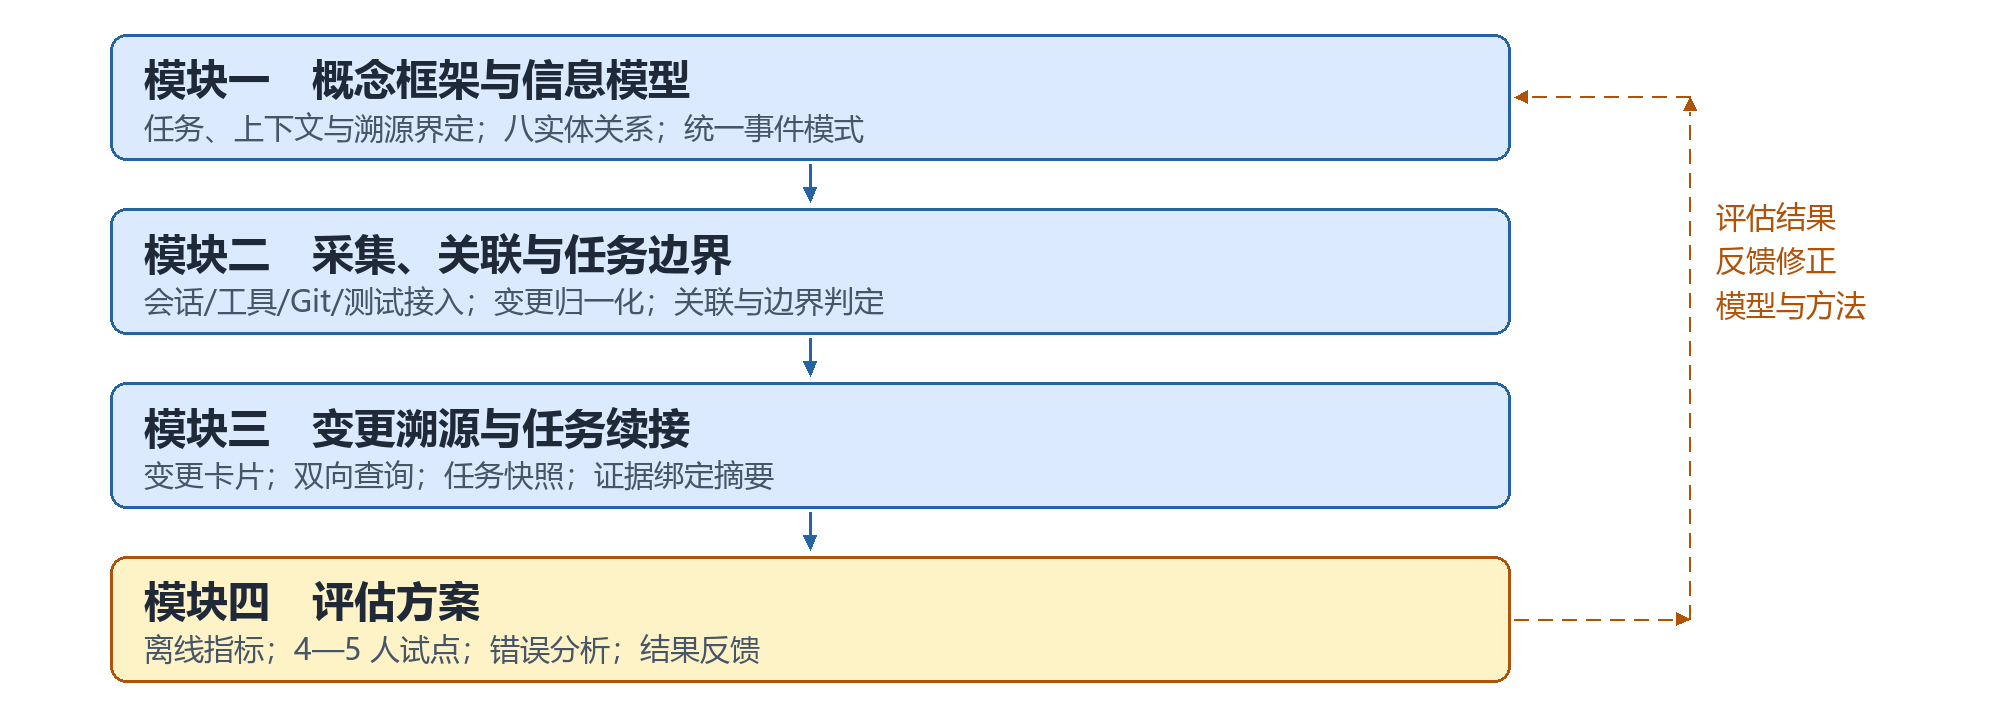
\includegraphics[width=\linewidth]{figures/fig1-route.png}
  \caption{研究技术路线}
  \label{fig:route}
\end{figure}

\tjformsubsub{（一）理论研究：任务上下文与变更溯源的概念框架}

本模块回答“研究对象是什么、依据何种标准判断方案有效”这一问题，构成 RQ1—RQ5 的概念前提。首先界定三个核心概念。开发任务（task）指开发者发起的一次有明确目标的开发工作单元，可包含多轮对话、多次文件修改、多次工具调用与多次测试执行。任务上下文（task context）指与某一任务相关的对话、变更、执行、测试、决策与未完成事项的集合。变更溯源（change provenance）指从一段代码变更出发，追溯其触发来源（用户请求或对话片段）、实施过程（工具调用）、验证依据（测试运行与结果）以及后续演化（回退、重写）的证据链。

在此基础上，本课题将任务上下文刻画为以任务为根的有向异构图 G=(V, E)：V 由开发任务、对话轮次、消息、工具调用、文件变更、测试运行、测试用例结果与检查点八类节点构成；E 由“包含”“触发”“产出”“验证”“演化”“快照”六类关系构成。变更溯源即在该图上从文件变更节点出发的可达性查询。该刻画导出四个待检验假设：H1，以任务为根的组织比以会话或文件为单位的组织更有利于恢复进展（RQ4）；H2，时间邻近、显式引用与文件级位置映射的组合足以恢复变更与对话之间的多对多关联（RQ2）；H3，任务边界可由空闲时长、显式指令、目标切换与提交动作联合判定（RQ5）；H4，要求结论绑定证据并以弃答作为兜底机制，可降低大模型结论的不支持率（RQ3）。

该框架与 PROV-O[32] 的映射如表~\ref{tab:prov} 所示。未直接采用 PROV 的原因在于：PROV 提供了实体、活动与代理的通用抽象，但未规定任务边界如何判定、hunk 如何与消息建立多对多关联、测试结果如何作为验证依据与变更建立关联；本课题的八实体模型是在 PROV 之上的领域特化。

\begin{table}[H]
  \centering
  \caption{信息模型与 PROV-O 的映射}
  \label{tab:prov}
  \begin{tabularx}{\linewidth}{@{}ll>{\raggedright\arraybackslash}X@{}}
    \toprule
    本课题概念 & PROV-O 对应 & 说明 \\
    \midrule
    开发任务 & prov:Activity & 以目标为边界的一段过程 \\
    对话轮次、消息 & prov:Entity & 用户或智能体产生的文本实体 \\
    工具调用 & prov:Activity & 使用工具的活动，prov:used 指向参数 \\
    文件变更（hunk） & prov:Entity & 由工具调用经 prov:wasGeneratedBy 生成 \\
    测试运行 & prov:Activity & 验证活动，prov:used 指向被验证的变更 \\
    测试用例结果 & prov:Entity & 验证活动的产出 \\
    智能体、开发者 & prov:Agent & 经 prov:wasAssociatedWith 关联活动 \\
    检查点 & prov:Entity & 任务阶段性快照 \\
    \bottomrule
  \end{tabularx}
\end{table}

最后，本模块建立覆盖表示、关联、溯源、恢复与大模型五个层面的 M1—M11 评价标准（见表~\ref{tab:metrics}），并将其作为后续模块的设计约束。

\tjformsubsub{（二）数据模型：任务中心实体关系与可扩展事件模式}

本模块将概念框架转化为可存储、可查询的表示，对应 RQ1，形成实体关系模型、事件模式与存储模式。实体关系如图~\ref{fig:model} 所示：开发任务为根节点，向下包含对话轮次，轮次包含消息；消息触发工具调用，工具调用产出文件变更（以 hunk 为单位）；文件变更由测试运行验证，测试运行产出测试用例结果；检查点记录任务在某一时刻的快照。所有记录均以任务标识为外键，从而支持“从任务聚合”与“从 hunk 反查”两个方向。

\begin{figure}[H]
  \centering
  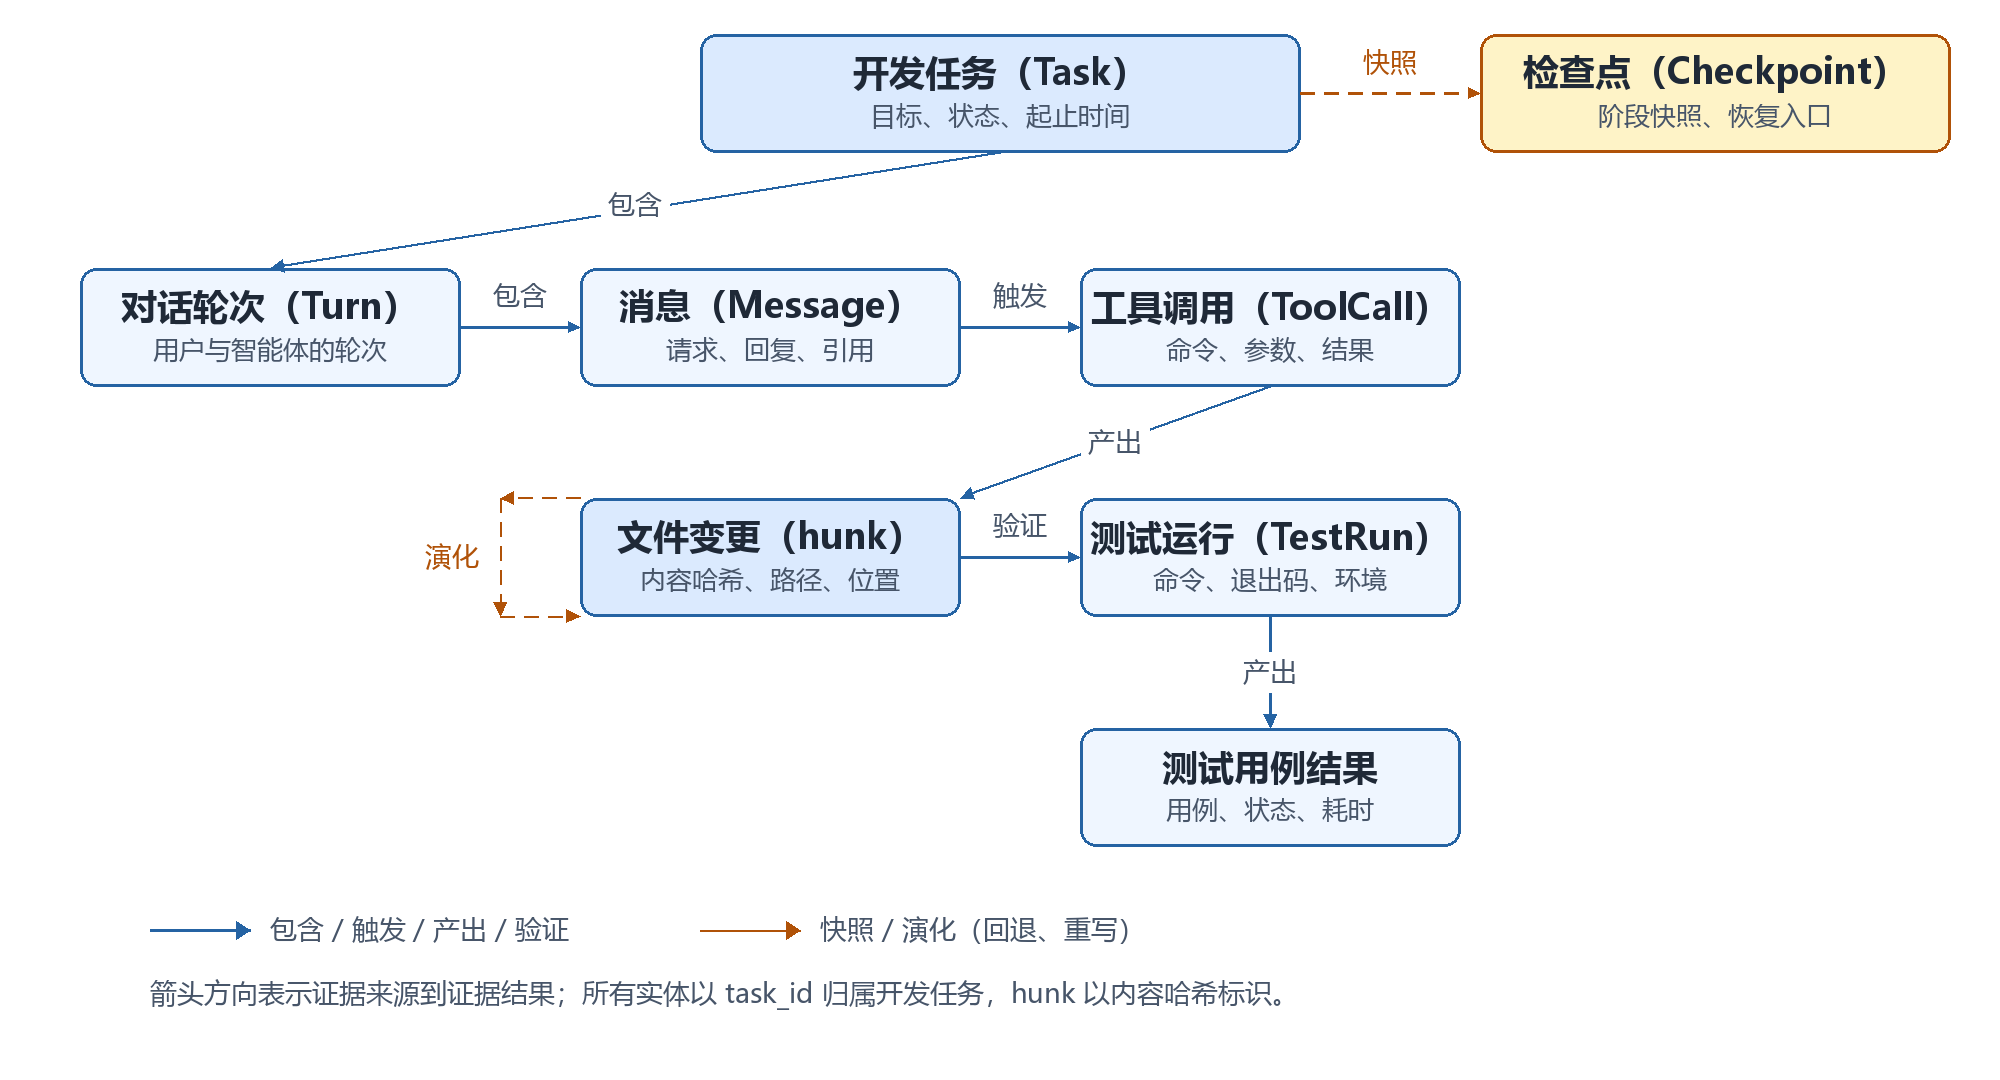
\includegraphics[width=\linewidth]{figures/fig2-model.png}
  \caption{任务中心实体关系与溯源关系}
  \label{fig:model}
\end{figure}

事件采用 JSON 表示，记为 e=(id, type, t, actor, source, payload, links)：id 为全局唯一标识，type 取自可扩展的类型注册表，t 为事件时间，actor 为开发者或智能体，source 标识事件来源，payload 保存原始字段，links 指向由该事件直接关联的实体。字段命名参考 OpenTelemetry 生成式 AI 语义约定[40]，同时保留原始字段，以避免因标准演进造成信息丢失。可扩展性由类型注册表保证：新增事件来源时仅需注册类型与字段映射，无须修改既有实体。

模型须满足三条不变量。其一，变更标识采用“内容哈希 + 文件路径 + 生成时间”三元组，行号仅作为属性而非标识，从而在行号漂移后仍能定位同一变更。其二，消息与 hunk 的关联为多对多关系：一条消息可促成多个 hunk，一个 hunk 也可能由多轮消息共同促成；关联区分 primary（工具调用直接产出该 hunk）与 secondary（消息提及该 hunk 涉及的文件或符号）。其三，测试结果必须同时指向被验证的变更与产生该变更的测试运行，使“哪次测试验证了哪次修改”可被查询。

存储采用关系表与全文索引相结合的方式：实体表保存规范化字段，关联表保存多对多关系，全文索引支持对话与变更卡片的中文检索；中文检索使用 trigram 分词器而非默认分词器，以避免整段中文被当作一个词。模型的有效性通过 M1（事件类型覆盖率）与 M2（文件级位置映射成功率）检验，并以 fixtures 固化样例、以模式校验脚本防止字段漂移。

\clearpage
\tjformsubsub{（三）算法与方法设计}

本模块设计四个核心算法与一个约束机制，分别对应 RQ2、RQ5 与 RQ3（含大模型部分）。设计遵循两条原则：一是在小样本条件下优先选择可解释、可人工复核的规则化方法，而非依赖大规模标注；二是每个算法均定义可测量的评价口径，使方案可被证伪。

\textbf{（1）编辑动作归一化与位置映射。}智能体的编辑动作与 unified diff 并不一致：Claude Code 的 Edit 采用“旧串→新串”形式，部分工具输出补丁，部分工具则整文件写入或使用搜索替换块。为此设计六步归一化：获取工具调用原始参数；在修改前文件中定位被替换片段（精确匹配失败时以首尾锚定结合模糊匹配）；应用替换得到修改后内容；对修改前后内容计算 unified diff 得到 hunk；与 Git 差异交叉校验，不一致时降低置信度；记录编辑格式元数据。归一化的正确性以 Git 差异为参照，采用 hunk 行区间与 Git 行区间的交并比（IoU）度量；需处理片段多次出现、换行符差异、跨函数替换与被格式化工具二次修改四类情形。语法感知的符号定位可借助 tree-sitter[41] 一类解析器完成，用于将 hunk 映射到函数或类。该算法在精确匹配下为线性时间，模糊匹配的最坏情形为二次时间，并通过首尾锚定将实际匹配长度控制在局部窗口内。

\textbf{（2）变更—对话关联。}给定消息集合 M 与 hunk 集合 H，为每个 (m, h) 对计算关联得分：对时间邻近、显式引用、文件级位置映射与文本相似度四项加权求和，其中显式引用包括路径、符号、行号、命令与测试名；得分超过预设阈值的候选进入关联集合，并输出置信度供人工确认。由于缺少大规模标注，权重与阈值在小规模验证集上调整，并报告阈值敏感性。关联为多对多关系，变更卡片展开 primary、折叠 secondary 并显示计数。评价在 20—30 对人工核对样本上进行，报告 top-1 准确率（M3）与错误类型分布；错误类型预先编码为时间邻近误配、行号漂移、多轮共同促成、并行任务交叉、工具调用无显式引用与模型编造六类。

\textbf{（3）任务边界判定。}将事件流切分为任务，等价于在时间轴上识别任务边界。候选特征包括空闲时长、显式指令（如“开始新任务”“换个问题”）、目标切换（文件或符号集合的显著变化）与提交动作。采用规则打分而非无监督聚类，原因有二：小样本条件下聚类结果不稳定且难以解释；边界判定需向开发者展示判断依据。边界判定在 6—8 个任务上以 F1（M4）评价，容差为 ±1 条消息，并报告阈值变化对 F1 的影响。

\textbf{（4）证据链构建与双向查询。}为每个 hunk 生成变更卡片，记录触发消息、工具调用、修改前后快照、验证测试与后续演化。查询分为两类：由代码到原因，输入 hunk 标识，返回触发消息、工具调用与验证测试；由原因到代码，输入消息或测试标识，返回其影响的 hunk 集合。查询在任务上下文图上进行 1—2 跳遍历，时间复杂度与节点度数相关；通过 hunk 标识、文件路径、消息标识与测试标识上的索引控制响应时间。评价使用 15 条预注册查询，以证据链同时包含金标准触发消息与验证测试为正确（M5），并报告 1 万条事件规模下的 P95 响应时间（M10）。

\textbf{（5）受证据约束的大模型摘要。}任务摘要与进展整理由大语言模型生成，但输出须遵循“结论 + 证据标识”的结构：每条结论必须给出支撑该结论的消息、hunk 或测试标识；生成后进行校验，检查证据是否存在、结论是否得到证据支持（结合词汇重叠与蕴含判断）；校验失败则弃答，而非给出无依据的结论。评价同时报告不支持率与弃答率（M6）：仅报告不支持率会诱导模型减少回答，仅报告弃答率则会掩盖错误，二者必须并列报告。

\tjformsubsub{（四）原型功能与交互设计}

本模块将前三个模块的能力转化为开发者可用的交互，对应 RQ4，并服务于 RQ1—RQ3 的观察。原型限定为三个核心视图。任务中心列出进行中、已完成与中断的任务，显示进展摘要、未完成项与待验证修改的数量，并提供“继续任务”的入口。任务时间线按时间顺序呈现对话轮次、工具调用、文件变更与测试运行，支持按文件、符号与测试名过滤；文件与代码片段视角并非第四个视图，而是时间线的过滤条件与详情呈现。变更证据侧栏在选中某个 hunk 后展示其变更卡片，并可沿“触发—实施—验证—演化”关系进行 1—2 跳跳转。

任务快照是续接功能的核心。快照由任务上下文图自动生成，将事项分为三类：已完成（有通过的测试支撑）、未完成（已提出但尚未实施）与待验证（测试失败或尚未运行）。每类事项均带有指向证据的链接，开发者可从摘要直接跳转至对应的消息、hunk 或测试结果，无须重新阅读全部记录。该设计依据任务上下文与恢复线索研究[23,27-28]，并借鉴 Whyline[34] 以“为什么”式提问组织证据的思路。

原型以 Web 形态实现（React 与 Vite），采用本地服务与 SQLite 存储，支持离线样例与回放，便于在答辩环境中复现；事件接入以 Claude Code 的官方钩子与 stream-json 为主，本地 JSONL 作为后备通道，Git 与测试报告作为补充来源。交互设计同时服务于评估：视图内记录操作日志与用时，供实验二分析。

\tjformsubsub{（五）评估验证方案}

本模块检验前四个模块的假设，对应 RQ1—RQ5。研究定位为小样本探索性预研（pilot）：4—5 名受试者、6—8 个任务，样本量不足以支撑确证性检验，故不设显著性结论，也不进行多重比较校正；全部推断以描述统计与逐人差值表述，并标注“探索性”，将研究资源集中于离线指标与错误分析。分析单位定为受试者而非单次观测。

实验一为离线客观评测，在 2 个中小规模开源仓库（TypeScript 与 Python 各 1 个）的 6—8 个任务上进行；任务覆盖缺陷修复、功能新增与代码重构三类，其中不少于三分之一改写自 SWE-bench Verified 与 SWE-rebench[42] 的真实 issue，其余为自行构造，并预先给出预期变更文件与验证测试。评测内容包括：20—30 对人工核对样本上的关联准确率；15 条预注册查询上的溯源正确率（查询与金标准在实验前写入版本库并提交哈希）；6—8 个任务上的边界判定与阈值敏感性；1 万条事件库上的查询性能；50 条大模型结论上的不支持率与弃答率。

实验二为受试者实验：4—5 名具备编程经验的同专业学生，在自我中断情境下完成 2 个任务（B0 与 C2 各 1 个），并回答恢复性问题与 SUS 问卷[43]；NASA-TLX[44] 作为可选的认知负荷观察。B0 为基线条件，受试者查看 Git 日志与差异、原始会话记录与测试报告；C2 为完整系统，包含证据链、跳转与任务快照。采用自我中断而非“第三方接手”情境，因为后者与真实场景并不等价；第三方接手范式仅作补充观察。每人一次到访约 90 分钟：任务各 30 分钟、条件间 10 分钟洗脱、说明与问卷 20 分钟；4—5 次到访共约 6—8 小时。

评价指标、定义与报告方式如表~\ref{tab:metrics} 所示。表中不设“达标线”列：在探索性定位下，硬阈值既不能构成结论依据，也容易掩盖区间信息；SUS 为必做的主观指标，NASA-TLX 为可选的认知负荷观察，二者均作描述性报告。分类指标报告比例与 Wilson 区间；受试者指标报告逐人差值点图、中位数与范围；样本量为 4—5 人，不进行推断统计。

\begin{longtable}{@{}>{\centering\arraybackslash}p{1.0cm}>{\raggedright\arraybackslash}p{2.5cm}>{\raggedright\arraybackslash}p{7.3cm}>{\raggedright\arraybackslash}p{2.6cm}@{}}
  \caption{评价指标定义与报告方式}\label{tab:metrics}\\
  \toprule
  编号 & 指标 & 定义与口径 & 报告方式 \\
  \midrule
  \endfirsthead
  \tjlongtablecont{4}
  \toprule
  编号 & 指标 & 定义与口径 & 报告方式 \\
  \midrule
  \endhead
  \bottomrule
  \endfoot
  M1 & 事件类型覆盖率 & 模式覆盖的记录类型数 ÷ Claude Code 官方文档列出的类型数与 Git/测试记录类型总数（分母预先固定） & 比例 + 区间 \\
  M2 & 文件级位置映射成功率 & 归一化后的编辑动作中，能与 Git 差异在同一文件同一行区间对齐的比例（以 Git 为参照） & 比例 + 分层 \\
  M3 & 关联准确率 & 20—30 对人工核对样本中，系统 top-1 关联与人工判断一致的比例 & 比例 + 错误类型 \\
  M4 & 任务边界判定 F1 & 系统切分边界与人工标注边界在 ±1 条消息容差内的重合度（6—8 个任务） & F1 + 阈值敏感性 \\
  M5 & 溯源查询正确率 & 15 条预注册查询中，证据链同时含金标准触发消息与验证测试的查询占比（二元判定） & 比例 + Wilson 区间 \\
  M6 & 不支持率与弃答率 & 50 条大模型结论中，证据不存在或语义不支持的比例，及同期弃答比例 & 双指标并列 \\
  M7 & 任务恢复用时 & 4—5 名受试者阅读上下文并回答恢复性问题的用时（秒），B0/C2 逐人对比 & 逐人差值 + 中位数 \\
  M8 & 理解要点命中数 & 回答命中金标准要点的个数（0—5），要点由未参与实现者预先列出并冻结 & 逐人差值 \\
  M9 & 问题定位用时 & 从给定修改请求到受试者指出正确目标文件与函数的用时（秒） & 逐人差值 \\
  M10 & 查询响应时间 & 1 万条事件下时间线首屏、1—2 跳证据链、中文检索的 P95（不含大模型） & 分查询类型 P50/P95 \\
  M11 & SUS 可用性评分 & 4—5 名受试者对系统的 SUS 评分（0—100） & 逐人得分 + 中位数 \\
  \end{longtable}

错误分析从实验一中抽取 20 个失败案例，由两名编码人员按六类编码报告占比与典型案例。效度威胁主要有四类：自构造任务可能引入实验者偏差，通过引入三分之一外部 issue 并采用“构造—执行—标注—评测”分离加以缓解；单机单用户场景限制结论外推；受试者为同专业同学，与研究者存在从属关系，故由第三方招募、不涉及课程成绩，且受试者可无理由退出；样本量 n=4—5 无法排除个体差异，结论限于方向性判断。研究伦理方面，受试者签署知情同意书；在数据入库前进行密钥与令牌过滤，匿名编号，并将映射表加密后单独保存；向第三方模型服务发送代码前进行过滤，并在界面中明示，同时提供本地模型或规则版摘要作为离线后备方案。

\clearpage
\tjformsubsection{3．工作进度安排}

本课题按任务书的教学周安排推进，六个阶段如表~\ref{tab:schedule} 与图~\ref{fig:gantt} 所示。第 9 周进行开题答辩，开题材料在第 8 周前完成；中期检查与答辩按学院统一安排。时间安排以教学周计，具体以学院通知为准。

\begin{table}[H]
  \centering
  \caption{研究进度安排}
  \label{tab:schedule}
  \begin{tabularx}{\linewidth}{@{}>{\raggedright\arraybackslash}p{3.2cm}>{\centering\arraybackslash}p{1.4cm}>{\raggedright\arraybackslash}X>{\raggedright\arraybackslash}p{3.2cm}@{}}
    \toprule
    阶段 & 教学周 & 主要工作 & 阶段成果 \\
    \midrule
    1　文献研究与产品调研 & 1—8 & 文献综述与竞品分析；确定研究问题、评价标准与实验任务；完成开题报告与答辩准备 & 文献综述、开题报告 \\
    2　关键方法设计与实现 & 9—14 & 信息模型与事件模式、编辑动作归一化、关联与边界判定、证据链查询 & 方法设计、实验脚本 \\
    3　系统设计与实现 & 15—20 & 三个视图、任务快照与续接、大模型摘要与证据校验、原型集成 & 原型 v0.9 \\
    4　系统验证与测试 & 21—22 & 6—8 个典型任务实验、4—5 人试点、错误分析与效度检查 & 实验数据、评估报告 \\
    5　毕业设计论文撰写 & 23—28 & 实验分析、论文初稿、图表与复现材料 & 论文初稿 \\
    6　论文审阅与修改 & 29—32 & 论文修改、查重、定稿与答辩材料 & 论文定稿、答辩材料 \\
    \bottomrule
  \end{tabularx}
\end{table}

\begin{figure}[H]
  \centering
  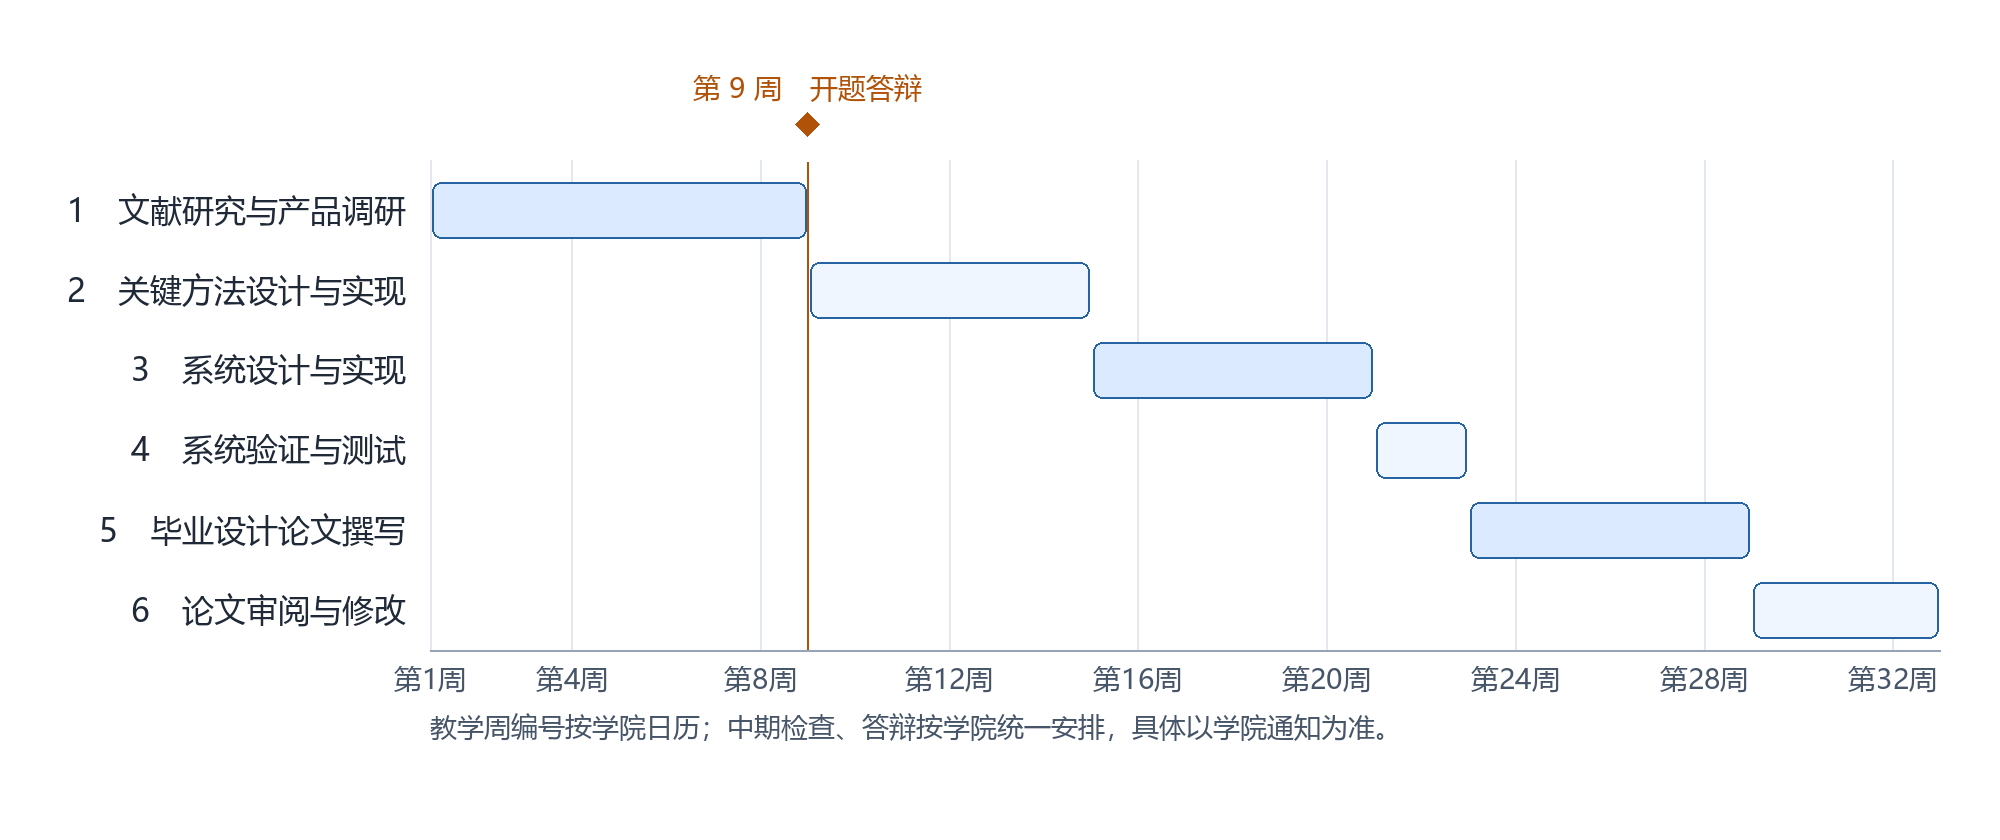
\includegraphics[width=\linewidth]{figures/fig3-gantt.png}
  \caption{研究进度甘特图}
  \label{fig:gantt}
\end{figure}

\clearpage
\tjformsection{三、\tjheadertext 的主要参考文献}\tjformsecnum{3}

（说明：会议文献按 GB/T 7714-2015 著录，出版地与出版者从略；网络资源引用日期统一为 2026-10-27。）

% 文献表按 Word 定稿：五号（10.5pt）、单倍行距；tjreflist 本身不设字号，故在此包一层。
{\zihao{5}\linespread{1}\selectfont\raggedright
\begin{tjreflist}
\item JIMENEZ C E, YANG J, WETTIG A, et al. SWE-bench: can language models resolve real-world GitHub issues?[C]//Proceedings of the 12th International Conference on Learning Representations. 2024. arXiv: 2310.06770.
\item CHEN M, TWOREK J, JUN H, et al. Evaluating large language models trained on code[EB/OL]. (2021-07-07)[2026-10-27]. https://arxiv.org/abs/2107.03374.
\item YANG J, JIMENEZ C E, WETTIG A, et al. SWE-agent: agent-computer interfaces enable automated software engineering[C]//Advances in Neural Information Processing Systems 37. 2024. arXiv: 2405.15793.
\item WANG X, LI B, SONG Y, et al. OpenHands: an open platform for AI software developers as generalist agents[C]//Proceedings of the 13th International Conference on Learning Representations. 2025. arXiv: 2407.16741.
\item WANG X, CHEN Y, YUAN L, et al. Executable code actions elicit better LLM agents[C]//Proceedings of the 41st International Conference on Machine Learning. 2024. arXiv: 2402.01030.
\item HONG S, ZHUGE M, CHEN J, et al. MetaGPT: meta programming for a multi-agent collaborative framework[C]//Proceedings of the 12th International Conference on Learning Representations. 2024. arXiv: 2308.00352.
\item QIAN C, LIU W, LIU H, et al. ChatDev: communicative agents for software development[C]//Proceedings of the 62nd Annual Meeting of the Association for Computational Linguistics. 2024: 15174-15186. DOI: 10.18653/v1/2024.acl-long.810.
\item XIA C S, DENG Y, DUNN S, et al. Agentless: demystifying LLM-based software engineering agents[EB/OL]. (2024-07-01)[2026-10-27]. https://arxiv.org/abs/2407.01489.
\item HOU X, ZHAO Y, LIU Y, et al. Large language models for software engineering: a systematic literature review[J]. ACM Transactions on Software Engineering and Methodology, 2024, 33(8). DOI: 10.1145/3695988.
\item FAN A, GOKKAYA B, HARMAN M, et al. Large language models for software engineering: survey and open problems[EB/OL]. (2023-10-05)[2026-10-27]. https://arxiv.org/abs/2310.03533.
\item 张犬俊, 谢杨, 房春荣, 等. 检索增强生成在软件工程中的应用综述[J]. 软件学报, 2026, 37(3): 1316-1339. DOI: 10.13328/j.cnki.jos.007567.
\item 汪莹, 字千成, 彭鑫, 等. 基于大语言模型的故障复现测试用例生成方法[J]. 软件学报, 2026, 37(4): 1690-1714. DOI: 10.13328/j.cnki.jos.007474.
\item PENG S, KALLIAMVAKOU E, CIHON P, et al. The impact of AI on developer productivity: evidence from GitHub Copilot[EB/OL]. (2023-02-13)[2026-10-27]. https://arxiv.org/abs/2302.06590.
\item MOZANNAR H, BANSAL G, FOURNEY A, et al. Reading between the lines: modeling user behavior and costs in AI-assisted programming[C]//Proceedings of the CHI Conference on Human Factors in Computing Systems. 2024: 1-16. DOI: 10.1145/3613904.3641936.
\item PERRY N, SRIVASTAVA M, KUMAR D, et al. Do users write more insecure code with AI assistants?[C]//Proceedings of the 2023 ACM SIGSAC Conference on Computer and Communications Security. 2023: 2785-2799. DOI: 10.1145/3576915.3623157.
\item BARKE S, JAMES M B, POLIKARPOVA N. Grounded Copilot: how programmers interact with code-generating models[J]. Proceedings of the ACM on Programming Languages, 2023, 7(OOPSLA1): 85-111. DOI: 10.1145/3586030.
\item VAITHILINGAM P, ZHANG T, SO S. Expectation vs. experience: evaluating the usability of code generation tools powered by large language models[C]//Proceedings of the CHI Conference on Human Factors in Computing Systems Extended Abstracts. 2022: 1-7. DOI: 10.1145/3491101.3519665.
\item ŚLIWERSKI J, ZIMMERMANN T, ZELLER A. When do changes induce fixes?[C]//Proceedings of the 2005 International Workshop on Mining Software Repositories. 2005: 1-5. DOI: 10.1145/1083142.1083147.
\item KAGDI H, COLLARD M L, MALETIC J I. A survey and taxonomy of approaches for mining software repositories in the context of software evolution[J]. Journal of Software Maintenance and Evolution: Research and Practice, 2007, 19(2): 77-131. DOI: 10.1002/smr.344.
\item ROBBES R, LANZA M. A change-based approach to software evolution[J]. Electronic Notes in Theoretical Computer Science, 2007, 166: 93-109. DOI: 10.1016/j.entcs.2006.06.015.
\item FALLERI J R, MORANDAT F, BLANC X, et al. Fine-grained and accurate source code differencing[C]//Proceedings of the 29th ACM/IEEE International Conference on Automated Software Engineering. 2014: 313-324. DOI: 10.1145/2642937.2642982.
\item GRUND F, CHOWDHURY S A, BRADLEY N C, et al. CodeShovel: constructing method-level source code histories[C]//Proceedings of the 43rd International Conference on Software Engineering. 2021: 1510-1522. DOI: 10.1109/ICSE43902.2021.00135.
\item KERSTEN M, MURPHY G C. Using task context to improve programmer productivity[C]//Proceedings of the 14th ACM SIGSOFT International Symposium on Foundations of Software Engineering. 2006: 1-11. DOI: 10.1145/1181775.1181777.
\item DRAGUNOV A N, DIETTERICH T G, JOHNSRUDE K, et al. TaskTracer: a desktop environment to support multi-tasking knowledge workers[C]//Proceedings of the 10th International Conference on Intelligent User Interfaces. 2005: 75-82. DOI: 10.1145/1040830.1040855.
\item BAO L, YE D, XING Z, et al. ActivitySpace: a remembrance framework to support interapplication information needs[C]//Proceedings of the 30th IEEE/ACM International Conference on Automated Software Engineering. 2015: 864-869. DOI: 10.1109/ASE.2015.90.
\item BEGEL A, KHOO Y P, ZIMMERMANN T. Codebook: discovering and exploiting relationships in software repositories[C]//Proceedings of the 32nd ACM/IEEE International Conference on Software Engineering. 2010: 125-134. DOI: 10.1145/1806799.1806821.
\item PARNIN C, RUGABER S. Resumption strategies for interrupted programming tasks[J]. Software Quality Journal, 2011, 19(1): 5-34. DOI: 10.1007/s11219-010-9104-9.
\item PARNIN C, DELINE R. Evaluating cues for resuming interrupted programming tasks[C]//Proceedings of the SIGCHI Conference on Human Factors in Computing Systems. 2010: 93-102. DOI: 10.1145/1753326.1753342.
\item SAFER I, MURPHY G C. Comparing episodic and semantic interfaces for task boundary identification[C]//Proceedings of the 2007 Conference of the Center for Advanced Studies on Collaborative Research. 2007: 229-243. DOI: 10.1145/1321211.1321235.
\item ROBBES R, LANZA M. Characterizing and understanding development sessions[C]//Proceedings of the 15th IEEE International Conference on Program Comprehension. 2007: 155-166. DOI: 10.1109/ICPC.2007.12.
\item CHENEY J, CHITICARIU L, TAN W C. Provenance in databases: why, how, and where[J]. Foundations and Trends in Databases, 2009, 1(4): 379-474. DOI: 10.1561/1900000006.
\item W3C. PROV-O: the PROV ontology[EB/OL]. (2013-04-30)[2026-10-27]. https://www.w3.org/TR/prov-o/.
\item SOUZA R, GUEROUDJI A, DEWITT S, et al. PROV-AGENT: unified provenance for tracking AI agent interactions in agentic workflows[C]//Proceedings of the 21st IEEE International Conference on e-Science. 2025. arXiv: 2508.02866.
\item KO A J, MYERS B A. Designing the Whyline: a debugging interface for asking questions about program behavior[C]//Proceedings of the SIGCHI Conference on Human Factors in Computing Systems. 2004: 151-158. DOI: 10.1145/985692.985712.
\item PIMENTEL J F, MURTA L, BRAGANHOLO V, et al. noWorkflow: a tool for collecting, analyzing, and managing provenance from Python scripts[J]. Proceedings of the VLDB Endowment, 2017, 10(12): 1841-1844. DOI: 10.14778/3137765.3137789.
\item Anthropic. Claude Code documentation: overview[EB/OL]. [2026-10-27]. https://code.claude.com/docs/en/overview.
\item Cursor. Cursor documentation[EB/OL]. [2026-10-27]. https://cursor.com/docs.
\item Cline. Cline: AI coding, open source and open choice[EB/OL]. [2026-10-27]. https://cline.bot.
\item Langfuse. Observability overview[EB/OL]. [2026-10-27]. https://langfuse.com/docs/observability/overview.
\item OpenTelemetry. Generative AI semantic conventions[EB/OL]. [2026-10-27]. https://opentelemetry.io/docs/specs/semconv/gen-ai/.
\item Tree-sitter. Tree-sitter documentation[EB/OL]. [2026-10-27]. https://tree-sitter.github.io/tree-sitter/.
\item BADERDINOV I, GOLUBEV A, NEKRASHEVICH M, et al. SWE-rebench: an automated pipeline for task collection and decontaminated evaluation of software engineering agents[EB/OL]. (2025-05-26)[2026-10-27]. https://arxiv.org/abs/2505.20411.
\item BROOKE J. SUS: a quick and dirty usability scale[M]//JORDAN P W, THOMAS B, WEERDMEESTER B A, et al. Usability Evaluation in Industry. London: Taylor \& Francis, 1996: 189-194.
\item HART S G, STAVELAND L E. Development of NASA-TLX (Task Load Index): results of empirical and theoretical research[J]. Advances in Psychology, 1988, 52: 139-183. DOI: 10.1016/S0166-4115(08)62386-9.
\end{tjreflist}
}

% 审核意见单独起页：两个意见框与“四、”标题合计超过一页余量，
% 不分页会把“专业审核意见”框挤到下一页，与 Word 版（审核意见独占末页）不一致。
\newpage
\tjformsection{四、审核意见}\tjformsecnum{4}

\begin{tjreviewbox}
  \tjformlabel{指导教师意见：}\tjformhint{（课题难度是否适中、工作量是否饱满、进度安排是否合理、工作条件是否具备、是否同意开题等）}

  \vspace{8\baselineskip}
  \tjformsignature{指导教师签名}{8em}
\end{tjreviewbox}

\begin{tjreviewbox}
  \tjformlabel{专业审核意见：}\tjformhint{（适当对各项内容给与意见和评价，字数不限。）}

  \vspace{6\baselineskip}
  \tjformsignature{负责人签名}{8em}
\end{tjreviewbox}
